

\tikzset{every picture/.style={line width=0.75pt}} %set default line width to 0.75pt        

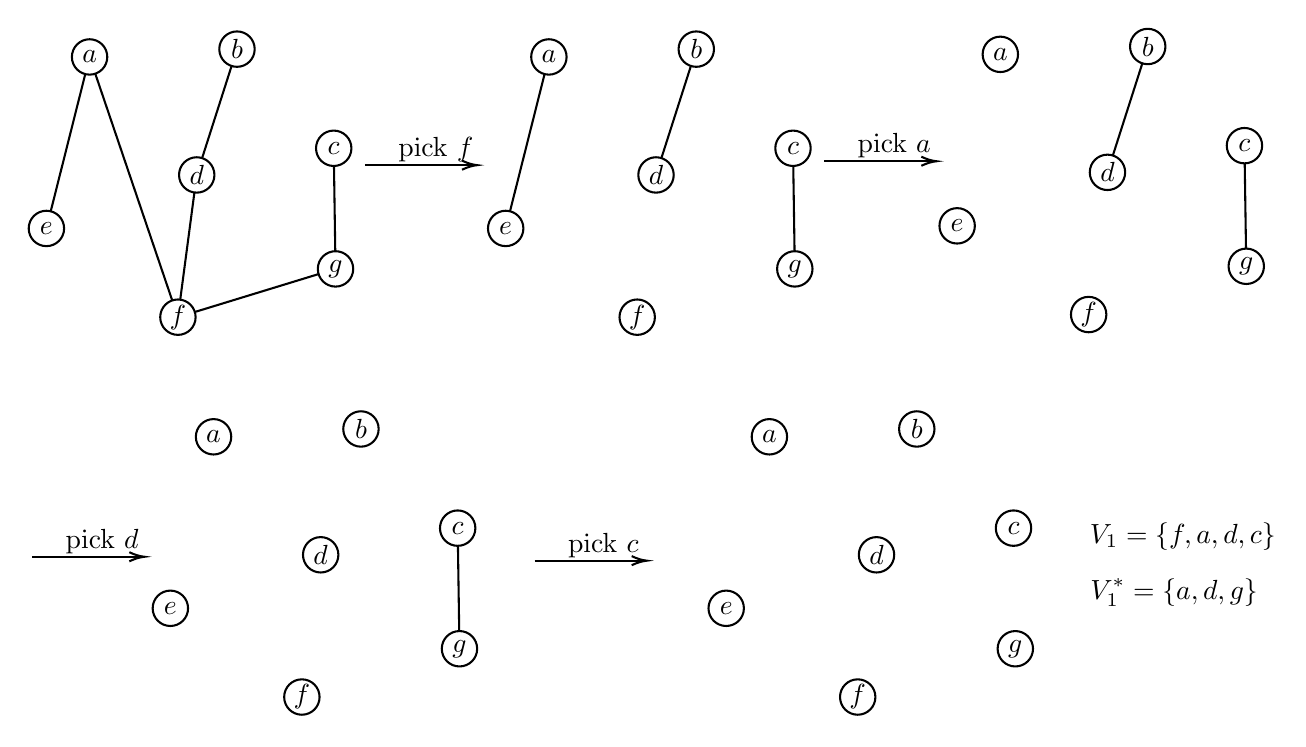
\begin{tikzpicture}[x=0.5pt,y=0.5pt,yscale=-1,xscale=1]
%uncomment if require: \path (0,509); %set diagram left start at 0, and has height of 509

%Straight Lines [id:da3853598268579197] 
\draw    (153.31,18.18) -- (124.22,109.11) ;
%Straight Lines [id:da21713072329995364] 
\draw    (224.52,177.01) -- (223.22,89.84) ;
%Straight Lines [id:da5478715757735835] 
\draw    (110.62,211.9) -- (224.52,177.01) ;
%Straight Lines [id:da42879006771456607] 
\draw    (46.79,23.83) -- (110.62,211.9) ;
%Straight Lines [id:da6771300098351073] 
\draw    (15.58,147.77) -- (46.79,23.83) ;
%Straight Lines [id:da4776548669152245] 
\draw    (110.62,211.9) -- (124.22,109.11) ;
%Shape: Ellipse [id:dp651117123053256] 
\draw  [fill={rgb, 255:red, 255; green, 255; blue, 255 }  ,fill opacity=1 ] (34,23.83) .. controls (34,16.77) and (39.73,11.04) .. (46.79,11.04) .. controls (53.86,11.04) and (59.58,16.77) .. (59.58,23.83) .. controls (59.58,30.9) and (53.86,36.62) .. (46.79,36.62) .. controls (39.73,36.62) and (34,30.9) .. (34,23.83) -- cycle ;
%Shape: Ellipse [id:dp7399561756845123] 
\draw  [fill={rgb, 255:red, 255; green, 255; blue, 255 }  ,fill opacity=1 ] (140.52,18.18) .. controls (140.52,11.11) and (146.25,5.39) .. (153.31,5.39) .. controls (160.38,5.39) and (166.1,11.11) .. (166.1,18.18) .. controls (166.1,25.24) and (160.38,30.97) .. (153.31,30.97) .. controls (146.25,30.97) and (140.52,25.24) .. (140.52,18.18) -- cycle ;
%Shape: Ellipse [id:dp8268258265249401] 
\draw  [fill={rgb, 255:red, 255; green, 255; blue, 255 }  ,fill opacity=1 ] (210.43,89.84) .. controls (210.43,82.78) and (216.15,77.05) .. (223.22,77.05) .. controls (230.28,77.05) and (236.01,82.78) .. (236.01,89.84) .. controls (236.01,96.9) and (230.28,102.63) .. (223.22,102.63) .. controls (216.15,102.63) and (210.43,96.9) .. (210.43,89.84) -- cycle ;
%Shape: Ellipse [id:dp5421818862330341] 
\draw  [fill={rgb, 255:red, 255; green, 255; blue, 255 }  ,fill opacity=1 ] (111.43,109.11) .. controls (111.43,102.05) and (117.15,96.32) .. (124.22,96.32) .. controls (131.28,96.32) and (137.01,102.05) .. (137.01,109.11) .. controls (137.01,116.18) and (131.28,121.9) .. (124.22,121.9) .. controls (117.15,121.9) and (111.43,116.18) .. (111.43,109.11) -- cycle ;
%Shape: Ellipse [id:dp45600813719389455] 
\draw  [fill={rgb, 255:red, 255; green, 255; blue, 255 }  ,fill opacity=1 ] (2.79,147.77) .. controls (2.79,140.71) and (8.52,134.98) .. (15.58,134.98) .. controls (22.64,134.98) and (28.37,140.71) .. (28.37,147.77) .. controls (28.37,154.84) and (22.64,160.56) .. (15.58,160.56) .. controls (8.52,160.56) and (2.79,154.84) .. (2.79,147.77) -- cycle ;
%Shape: Ellipse [id:dp031187496945339066] 
\draw  [fill={rgb, 255:red, 255; green, 255; blue, 255 }  ,fill opacity=1 ] (97.83,211.9) .. controls (97.83,204.83) and (103.56,199.11) .. (110.62,199.11) .. controls (117.69,199.11) and (123.41,204.83) .. (123.41,211.9) .. controls (123.41,218.96) and (117.69,224.69) .. (110.62,224.69) .. controls (103.56,224.69) and (97.83,218.96) .. (97.83,211.9) -- cycle ;
%Shape: Ellipse [id:dp7474313144054212] 
\draw  [fill={rgb, 255:red, 255; green, 255; blue, 255 }  ,fill opacity=1 ] (211.73,177.01) .. controls (211.73,169.94) and (217.46,164.22) .. (224.52,164.22) .. controls (231.59,164.22) and (237.31,169.94) .. (237.31,177.01) .. controls (237.31,184.07) and (231.59,189.8) .. (224.52,189.8) .. controls (217.46,189.8) and (211.73,184.07) .. (211.73,177.01) -- cycle ;
%Straight Lines [id:da10915523795701287] 
\draw    (485.24,18.18) -- (456.14,109.11) ;
%Straight Lines [id:da6013659372024278] 
\draw    (556.45,177.01) -- (555.14,89.84) ;
%Straight Lines [id:da2476997276246733] 
\draw    (347.5,147.77) -- (378.72,23.83) ;
%Shape: Ellipse [id:dp27040633021074256] 
\draw  [fill={rgb, 255:red, 255; green, 255; blue, 255 }  ,fill opacity=1 ] (365.93,23.83) .. controls (365.93,16.77) and (371.65,11.04) .. (378.72,11.04) .. controls (385.78,11.04) and (391.51,16.77) .. (391.51,23.83) .. controls (391.51,30.9) and (385.78,36.62) .. (378.72,36.62) .. controls (371.65,36.62) and (365.93,30.9) .. (365.93,23.83) -- cycle ;
%Shape: Ellipse [id:dp9153562797015269] 
\draw  [fill={rgb, 255:red, 255; green, 255; blue, 255 }  ,fill opacity=1 ] (472.45,18.18) .. controls (472.45,11.11) and (478.17,5.39) .. (485.24,5.39) .. controls (492.3,5.39) and (498.03,11.11) .. (498.03,18.18) .. controls (498.03,25.24) and (492.3,30.97) .. (485.24,30.97) .. controls (478.17,30.97) and (472.45,25.24) .. (472.45,18.18) -- cycle ;
%Shape: Ellipse [id:dp47379487417600374] 
\draw  [fill={rgb, 255:red, 255; green, 255; blue, 255 }  ,fill opacity=1 ] (542.35,89.84) .. controls (542.35,82.78) and (548.07,77.05) .. (555.14,77.05) .. controls (562.2,77.05) and (567.93,82.78) .. (567.93,89.84) .. controls (567.93,96.9) and (562.2,102.63) .. (555.14,102.63) .. controls (548.07,102.63) and (542.35,96.9) .. (542.35,89.84) -- cycle ;
%Shape: Ellipse [id:dp7207828118279439] 
\draw  [fill={rgb, 255:red, 255; green, 255; blue, 255 }  ,fill opacity=1 ] (443.35,109.11) .. controls (443.35,102.05) and (449.08,96.32) .. (456.14,96.32) .. controls (463.2,96.32) and (468.93,102.05) .. (468.93,109.11) .. controls (468.93,116.18) and (463.2,121.9) .. (456.14,121.9) .. controls (449.08,121.9) and (443.35,116.18) .. (443.35,109.11) -- cycle ;
%Shape: Ellipse [id:dp7155442322771159] 
\draw  [fill={rgb, 255:red, 255; green, 255; blue, 255 }  ,fill opacity=1 ] (334.71,147.77) .. controls (334.71,140.71) and (340.44,134.98) .. (347.5,134.98) .. controls (354.57,134.98) and (360.29,140.71) .. (360.29,147.77) .. controls (360.29,154.84) and (354.57,160.56) .. (347.5,160.56) .. controls (340.44,160.56) and (334.71,154.84) .. (334.71,147.77) -- cycle ;
%Shape: Ellipse [id:dp4818001756043101] 
\draw  [fill={rgb, 255:red, 255; green, 255; blue, 255 }  ,fill opacity=1 ] (429.75,211.9) .. controls (429.75,204.83) and (435.48,199.11) .. (442.54,199.11) .. controls (449.61,199.11) and (455.33,204.83) .. (455.33,211.9) .. controls (455.33,218.96) and (449.61,224.69) .. (442.54,224.69) .. controls (435.48,224.69) and (429.75,218.96) .. (429.75,211.9) -- cycle ;
%Shape: Ellipse [id:dp9764479331484588] 
\draw  [fill={rgb, 255:red, 255; green, 255; blue, 255 }  ,fill opacity=1 ] (543.66,177.01) .. controls (543.66,169.94) and (549.38,164.22) .. (556.45,164.22) .. controls (563.51,164.22) and (569.24,169.94) .. (569.24,177.01) .. controls (569.24,184.07) and (563.51,189.8) .. (556.45,189.8) .. controls (549.38,189.8) and (543.66,184.07) .. (543.66,177.01) -- cycle ;
%Straight Lines [id:da022074673171788572] 
\draw    (811.5,16.29) -- (782.4,107.23) ;
%Straight Lines [id:da7079754945425016] 
\draw    (882.71,175.12) -- (881.4,87.95) ;
%Shape: Ellipse [id:dp8120027238634924] 
\draw  [fill={rgb, 255:red, 255; green, 255; blue, 255 }  ,fill opacity=1 ] (692.19,21.95) .. controls (692.19,14.88) and (697.92,9.16) .. (704.98,9.16) .. controls (712.04,9.16) and (717.77,14.88) .. (717.77,21.95) .. controls (717.77,29.01) and (712.04,34.74) .. (704.98,34.74) .. controls (697.92,34.74) and (692.19,29.01) .. (692.19,21.95) -- cycle ;
%Shape: Ellipse [id:dp23465413123771173] 
\draw  [fill={rgb, 255:red, 255; green, 255; blue, 255 }  ,fill opacity=1 ] (798.71,16.29) .. controls (798.71,9.23) and (804.44,3.5) .. (811.5,3.5) .. controls (818.56,3.5) and (824.29,9.23) .. (824.29,16.29) .. controls (824.29,23.35) and (818.56,29.08) .. (811.5,29.08) .. controls (804.44,29.08) and (798.71,23.35) .. (798.71,16.29) -- cycle ;
%Shape: Ellipse [id:dp6697870946666823] 
\draw  [fill={rgb, 255:red, 255; green, 255; blue, 255 }  ,fill opacity=1 ] (868.61,87.95) .. controls (868.61,80.89) and (874.34,75.16) .. (881.4,75.16) .. controls (888.47,75.16) and (894.19,80.89) .. (894.19,87.95) .. controls (894.19,95.02) and (888.47,100.74) .. (881.4,100.74) .. controls (874.34,100.74) and (868.61,95.02) .. (868.61,87.95) -- cycle ;
%Shape: Ellipse [id:dp6678250120125151] 
\draw  [fill={rgb, 255:red, 255; green, 255; blue, 255 }  ,fill opacity=1 ] (769.61,107.23) .. controls (769.61,100.16) and (775.34,94.44) .. (782.4,94.44) .. controls (789.47,94.44) and (795.19,100.16) .. (795.19,107.23) .. controls (795.19,114.29) and (789.47,120.02) .. (782.4,120.02) .. controls (775.34,120.02) and (769.61,114.29) .. (769.61,107.23) -- cycle ;
%Shape: Ellipse [id:dp44880213332154095] 
\draw  [fill={rgb, 255:red, 255; green, 255; blue, 255 }  ,fill opacity=1 ] (660.98,145.89) .. controls (660.98,138.83) and (666.7,133.1) .. (673.77,133.1) .. controls (680.83,133.1) and (686.56,138.83) .. (686.56,145.89) .. controls (686.56,152.95) and (680.83,158.68) .. (673.77,158.68) .. controls (666.7,158.68) and (660.98,152.95) .. (660.98,145.89) -- cycle ;
%Shape: Ellipse [id:dp5261031453835676] 
\draw  [fill={rgb, 255:red, 255; green, 255; blue, 255 }  ,fill opacity=1 ] (756.02,210.01) .. controls (756.02,202.95) and (761.75,197.22) .. (768.81,197.22) .. controls (775.87,197.22) and (781.6,202.95) .. (781.6,210.01) .. controls (781.6,217.07) and (775.87,222.8) .. (768.81,222.8) .. controls (761.75,222.8) and (756.02,217.07) .. (756.02,210.01) -- cycle ;
%Shape: Ellipse [id:dp96264308088132] 
\draw  [fill={rgb, 255:red, 255; green, 255; blue, 255 }  ,fill opacity=1 ] (869.92,175.12) .. controls (869.92,168.06) and (875.65,162.33) .. (882.71,162.33) .. controls (889.77,162.33) and (895.5,168.06) .. (895.5,175.12) .. controls (895.5,182.18) and (889.77,187.91) .. (882.71,187.91) .. controls (875.65,187.91) and (869.92,182.18) .. (869.92,175.12) -- cycle ;
%Straight Lines [id:da5971152802941945] 
\draw    (314.1,451.53) -- (312.8,364.36) ;
%Shape: Ellipse [id:dp08371522903251905] 
\draw  [fill={rgb, 255:red, 255; green, 255; blue, 255 }  ,fill opacity=1 ] (123.58,298.35) .. controls (123.58,291.29) and (129.31,285.56) .. (136.37,285.56) .. controls (143.44,285.56) and (149.16,291.29) .. (149.16,298.35) .. controls (149.16,305.42) and (143.44,311.14) .. (136.37,311.14) .. controls (129.31,311.14) and (123.58,305.42) .. (123.58,298.35) -- cycle ;
%Shape: Ellipse [id:dp16754302978302682] 
\draw  [fill={rgb, 255:red, 255; green, 255; blue, 255 }  ,fill opacity=1 ] (230.11,292.7) .. controls (230.11,285.63) and (235.83,279.91) .. (242.9,279.91) .. controls (249.96,279.91) and (255.69,285.63) .. (255.69,292.7) .. controls (255.69,299.76) and (249.96,305.48) .. (242.9,305.48) .. controls (235.83,305.48) and (230.11,299.76) .. (230.11,292.7) -- cycle ;
%Shape: Ellipse [id:dp8803652600651565] 
\draw  [fill={rgb, 255:red, 255; green, 255; blue, 255 }  ,fill opacity=1 ] (300.01,364.36) .. controls (300.01,357.3) and (305.73,351.57) .. (312.8,351.57) .. controls (319.86,351.57) and (325.59,357.3) .. (325.59,364.36) .. controls (325.59,371.42) and (319.86,377.15) .. (312.8,377.15) .. controls (305.73,377.15) and (300.01,371.42) .. (300.01,364.36) -- cycle ;
%Shape: Ellipse [id:dp08434869719365379] 
\draw  [fill={rgb, 255:red, 255; green, 255; blue, 255 }  ,fill opacity=1 ] (201.01,383.63) .. controls (201.01,376.57) and (206.74,370.84) .. (213.8,370.84) .. controls (220.86,370.84) and (226.59,376.57) .. (226.59,383.63) .. controls (226.59,390.7) and (220.86,396.42) .. (213.8,396.42) .. controls (206.74,396.42) and (201.01,390.7) .. (201.01,383.63) -- cycle ;
%Shape: Ellipse [id:dp8697258636657205] 
\draw  [fill={rgb, 255:red, 255; green, 255; blue, 255 }  ,fill opacity=1 ] (92.37,422.29) .. controls (92.37,415.23) and (98.1,409.5) .. (105.16,409.5) .. controls (112.23,409.5) and (117.95,415.23) .. (117.95,422.29) .. controls (117.95,429.36) and (112.23,435.08) .. (105.16,435.08) .. controls (98.1,435.08) and (92.37,429.36) .. (92.37,422.29) -- cycle ;
%Shape: Ellipse [id:dp3796179832525568] 
\draw  [fill={rgb, 255:red, 255; green, 255; blue, 255 }  ,fill opacity=1 ] (187.41,486.42) .. controls (187.41,479.35) and (193.14,473.63) .. (200.2,473.63) .. controls (207.27,473.63) and (212.99,479.35) .. (212.99,486.42) .. controls (212.99,493.48) and (207.27,499.21) .. (200.2,499.21) .. controls (193.14,499.21) and (187.41,493.48) .. (187.41,486.42) -- cycle ;
%Shape: Ellipse [id:dp22651898621493904] 
\draw  [fill={rgb, 255:red, 255; green, 255; blue, 255 }  ,fill opacity=1 ] (301.32,451.53) .. controls (301.32,444.46) and (307.04,438.74) .. (314.1,438.74) .. controls (321.17,438.74) and (326.89,444.46) .. (326.89,451.53) .. controls (326.89,458.59) and (321.17,464.32) .. (314.1,464.32) .. controls (307.04,464.32) and (301.32,458.59) .. (301.32,451.53) -- cycle ;

%Shape: Ellipse [id:dp6886010266116899] 
\draw  [fill={rgb, 255:red, 255; green, 255; blue, 255 }  ,fill opacity=1 ] (525.29,298.35) .. controls (525.29,291.29) and (531.01,285.56) .. (538.08,285.56) .. controls (545.14,285.56) and (550.87,291.29) .. (550.87,298.35) .. controls (550.87,305.42) and (545.14,311.14) .. (538.08,311.14) .. controls (531.01,311.14) and (525.29,305.42) .. (525.29,298.35) -- cycle ;
%Shape: Ellipse [id:dp4406300893596924] 
\draw  [fill={rgb, 255:red, 255; green, 255; blue, 255 }  ,fill opacity=1 ] (631.81,292.7) .. controls (631.81,285.63) and (637.53,279.91) .. (644.6,279.91) .. controls (651.66,279.91) and (657.39,285.63) .. (657.39,292.7) .. controls (657.39,299.76) and (651.66,305.48) .. (644.6,305.48) .. controls (637.53,305.48) and (631.81,299.76) .. (631.81,292.7) -- cycle ;
%Shape: Ellipse [id:dp708253572812504] 
\draw  [fill={rgb, 255:red, 255; green, 255; blue, 255 }  ,fill opacity=1 ] (701.71,364.36) .. controls (701.71,357.3) and (707.43,351.57) .. (714.5,351.57) .. controls (721.56,351.57) and (727.29,357.3) .. (727.29,364.36) .. controls (727.29,371.42) and (721.56,377.15) .. (714.5,377.15) .. controls (707.43,377.15) and (701.71,371.42) .. (701.71,364.36) -- cycle ;
%Shape: Ellipse [id:dp12047908084857373] 
\draw  [fill={rgb, 255:red, 255; green, 255; blue, 255 }  ,fill opacity=1 ] (602.71,383.63) .. controls (602.71,376.57) and (608.44,370.84) .. (615.5,370.84) .. controls (622.56,370.84) and (628.29,376.57) .. (628.29,383.63) .. controls (628.29,390.7) and (622.56,396.42) .. (615.5,396.42) .. controls (608.44,396.42) and (602.71,390.7) .. (602.71,383.63) -- cycle ;
%Shape: Ellipse [id:dp06065835414250742] 
\draw  [fill={rgb, 255:red, 255; green, 255; blue, 255 }  ,fill opacity=1 ] (494.07,422.29) .. controls (494.07,415.23) and (499.8,409.5) .. (506.86,409.5) .. controls (513.93,409.5) and (519.65,415.23) .. (519.65,422.29) .. controls (519.65,429.36) and (513.93,435.08) .. (506.86,435.08) .. controls (499.8,435.08) and (494.07,429.36) .. (494.07,422.29) -- cycle ;
%Shape: Ellipse [id:dp7223087244252215] 
\draw  [fill={rgb, 255:red, 255; green, 255; blue, 255 }  ,fill opacity=1 ] (589.12,486.42) .. controls (589.12,479.35) and (594.84,473.63) .. (601.91,473.63) .. controls (608.97,473.63) and (614.69,479.35) .. (614.69,486.42) .. controls (614.69,493.48) and (608.97,499.21) .. (601.91,499.21) .. controls (594.84,499.21) and (589.12,493.48) .. (589.12,486.42) -- cycle ;
%Shape: Ellipse [id:dp483775428948783] 
\draw  [fill={rgb, 255:red, 255; green, 255; blue, 255 }  ,fill opacity=1 ] (703.02,451.53) .. controls (703.02,444.46) and (708.74,438.74) .. (715.81,438.74) .. controls (722.87,438.74) and (728.6,444.46) .. (728.6,451.53) .. controls (728.6,458.59) and (722.87,464.32) .. (715.81,464.32) .. controls (708.74,464.32) and (703.02,458.59) .. (703.02,451.53) -- cycle ;

%Straight Lines [id:da8565598108716722] 
\draw    (245.8,102.04) -- (324.89,102.04) ;
\draw [shift={(326.89,102.04)}, rotate = 180] [color={rgb, 255:red, 0; green, 0; blue, 0 }  ][line width=0.75]    (10.93,-3.29) .. controls (6.95,-1.4) and (3.31,-0.3) .. (0,0) .. controls (3.31,0.3) and (6.95,1.4) .. (10.93,3.29)   ;
%Straight Lines [id:da8466299980928367] 
\draw    (577.72,99.21) -- (656.82,99.21) ;
\draw [shift={(658.82,99.21)}, rotate = 180] [color={rgb, 255:red, 0; green, 0; blue, 0 }  ][line width=0.75]    (10.93,-3.29) .. controls (6.95,-1.4) and (3.31,-0.3) .. (0,0) .. controls (3.31,0.3) and (6.95,1.4) .. (10.93,3.29)   ;
%Straight Lines [id:da6943383967058451] 
\draw    (5.35,385.05) -- (84.44,385.05) ;
\draw [shift={(86.44,385.05)}, rotate = 180] [color={rgb, 255:red, 0; green, 0; blue, 0 }  ][line width=0.75]    (10.93,-3.29) .. controls (6.95,-1.4) and (3.31,-0.3) .. (0,0) .. controls (3.31,0.3) and (6.95,1.4) .. (10.93,3.29)   ;
%Straight Lines [id:da7622342093674817] 
\draw    (368.39,387.87) -- (447.48,387.87) ;
\draw [shift={(449.48,387.87)}, rotate = 180] [color={rgb, 255:red, 0; green, 0; blue, 0 }  ][line width=0.75]    (10.93,-3.29) .. controls (6.95,-1.4) and (3.31,-0.3) .. (0,0) .. controls (3.31,0.3) and (6.95,1.4) .. (10.93,3.29)   ;

% Text Node
\draw (767.36,358.13) node [anchor=north west][inner sep=0.75pt]   [align=left] {$\displaystyle V_{1} =\{f,a,d,c\}$};
% Text Node
\draw (767.82,398.59) node [anchor=north west][inner sep=0.75pt]   [align=left] {$\displaystyle V^{*}_{1} =\{a,d,g\}$};
% Text Node
\draw (46.79,23.83) node   [align=left] {$\displaystyle a$};
% Text Node
\draw (153.31,18.18) node   [align=left] {$\displaystyle b$};
% Text Node
\draw (223.22,89.84) node   [align=left] {$\displaystyle c$};
% Text Node
\draw (124.22,109.11) node   [align=left] {$\displaystyle d$};
% Text Node
\draw (15.58,147.77) node   [align=left] {$\displaystyle e$};
% Text Node
\draw (110.62,211.9) node   [align=left] {$\displaystyle f$};
% Text Node
\draw (224.52,177.01) node   [align=left] {$\displaystyle g$};
% Text Node
\draw (378.72,23.83) node   [align=left] {$\displaystyle a$};
% Text Node
\draw (485.24,18.18) node   [align=left] {$\displaystyle b$};
% Text Node
\draw (555.14,89.84) node   [align=left] {$\displaystyle c$};
% Text Node
\draw (456.14,109.11) node   [align=left] {$\displaystyle d$};
% Text Node
\draw (347.5,147.77) node   [align=left] {$\displaystyle e$};
% Text Node
\draw (442.54,211.9) node   [align=left] {$\displaystyle f$};
% Text Node
\draw (556.45,177.01) node   [align=left] {$\displaystyle g$};
% Text Node
\draw (704.98,21.95) node   [align=left] {$\displaystyle a$};
% Text Node
\draw (811.5,16.29) node   [align=left] {$\displaystyle b$};
% Text Node
\draw (881.4,87.95) node   [align=left] {$\displaystyle c$};
% Text Node
\draw (782.4,107.23) node   [align=left] {$\displaystyle d$};
% Text Node
\draw (673.77,145.89) node   [align=left] {$\displaystyle e$};
% Text Node
\draw (768.81,210.01) node   [align=left] {$\displaystyle f$};
% Text Node
\draw (882.71,175.12) node   [align=left] {$\displaystyle g$};
% Text Node
\draw (136.37,298.35) node   [align=left] {$\displaystyle a$};
% Text Node
\draw (242.9,292.7) node   [align=left] {$\displaystyle b$};
% Text Node
\draw (312.8,364.36) node   [align=left] {$\displaystyle c$};
% Text Node
\draw (213.8,383.63) node   [align=left] {$\displaystyle d$};
% Text Node
\draw (105.16,422.29) node   [align=left] {$\displaystyle e$};
% Text Node
\draw (200.2,486.42) node   [align=left] {$\displaystyle f$};
% Text Node
\draw (314.1,451.53) node   [align=left] {$\displaystyle g$};
% Text Node
\draw (538.08,298.35) node   [align=left] {$\displaystyle a$};
% Text Node
\draw (644.6,292.7) node   [align=left] {$\displaystyle b$};
% Text Node
\draw (714.5,364.36) node   [align=left] {$\displaystyle c$};
% Text Node
\draw (615.5,383.63) node   [align=left] {$\displaystyle d$};
% Text Node
\draw (506.86,422.29) node   [align=left] {$\displaystyle e$};
% Text Node
\draw (601.91,486.42) node   [align=left] {$\displaystyle f$};
% Text Node
\draw (715.81,451.53) node   [align=left] {$\displaystyle g$};
% Text Node
\draw (267.71,79.84) node [anchor=north west][inner sep=0.75pt]   [align=left] {pick $\displaystyle f$};
% Text Node
\draw (599.68,77.01) node [anchor=north west][inner sep=0.75pt]   [align=left] {pick $\displaystyle a$};
% Text Node
\draw (27.28,362.84) node [anchor=north west][inner sep=0.75pt]   [align=left] {pick $\displaystyle d$};
% Text Node
\draw (390.35,365.67) node [anchor=north west][inner sep=0.75pt]   [align=left] {pick $\displaystyle c$};


\end{tikzpicture}

